\section{Towards Weakly Supervised Temporal Uncertainty Localization}
\label{sec:non_static}

Mechanistic detectors face a tension between coverage and scalability.
Static probing classifiers \citep{azaria2023,orgad2024} operate on a
single layer-token position and ignore signal elsewhere in $A$; the
optimal position varies across samples, datasets, and LLMs, often
requiring an external search \citep{orgad2024}. Methods that process
the whole tensor capture distributed signal but are ill-suited to
real-time long-form generation: some pool the token axis into a fixed
size, diluting signal as responses grow; others remain accurate at
long context but require one forward per token. Even when a
full-tensor method does scale, a single sequence-level score does not
say where the suspicious activations lie, a poor fit for
responses where most tokens are correct and only a few are
problematic.

\paragraph{Tensor methods degrade with response length.}
Figure~\ref{fig:perf_by_length} reports per-token AUROC on LongFact as
the input prefix length $T$ grows. ACT-ViT with a short pooled token
axis performs well only for short prefixes, but its performance drops
as more generated tokens are compressed into the same fixed-size
representation; widening the pooled axis partially reduces this
collapse, but it still does not recover Temp-ViT's flatter performance
across response lengths. This supports our central design choice:
instead of compressing the whole response into one fixed activation
image, Temp-ViT scores local token windows and models their temporal
evolution.

\paragraph{Why windows instead of isolated tokens?} Hallucination
labels are usually available at the response, sentence, or claim level,
not at the exact token-window level. Moreover, the activation signal
is not confined to the hallucinated token itself.
Figure~\ref{fig:signal_propagation} measures this directly: on
RAGTruth, a linear probe's ROC-AUC ramps from chance at offset $-24$
to $0.66$ at the token immediately before a hallucinated span, rises
monotonically through the span ($0.71 \to 0.79$), and decays slowly
afterward. Adjacent context therefore carries useful uncertainty
signal, while direct token supervision would be noisy. We treat span
labels as weak supervision and learn to localize uncertainty through
window-level temporal modeling.

\begin{figure}[t]
\centering
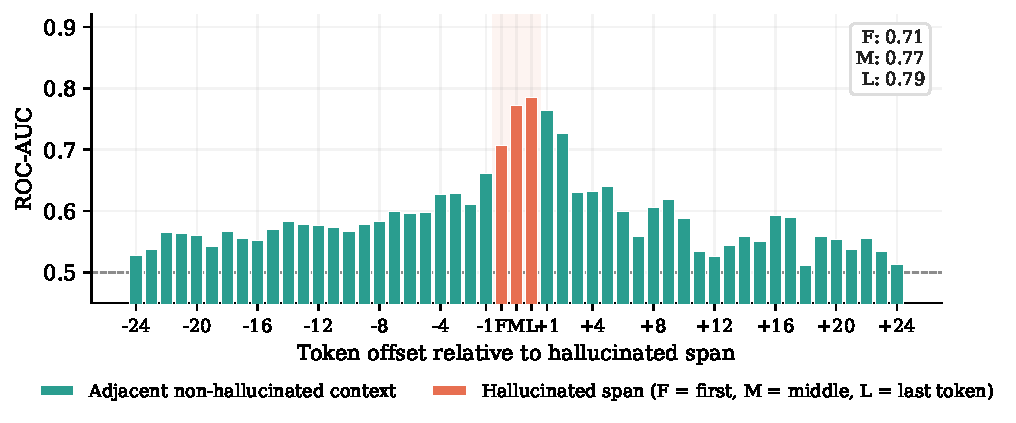
\includegraphics[width=0.95\linewidth]{figs/fig_signal_propagation.pdf}
\caption{Per-offset ROC-AUC of a linear probe (layer $L=1$ of the
$L=8$ pre-pooled hidden-state grid) measured on tokens at each offset
relative to a hallucinated span on RAGTruth (Llama-2-13b-chat). Teal
bars use the continuous non-hallucinated context adjacent to the span;
coral bars (F, M, L) are the first, middle, and last token of the
hallucinated span. Three regimes are visible: a pre-span ramp from
near-chance to AUC $\approx 0.66$ at offset $-1$ (anticipatory signal
one token ahead of the hallucination); a monotone in-span rise
$0.71 \to 0.79$; and post-span persistence that decays slowly back to
chance. The window-based localization of Section~\ref{sec:non_static}
exploits this neighborhood structure rather than treating tokens
independently.}
\label{fig:signal_propagation}
\end{figure}


\paragraph{Additional probe evidence.} Per layer-token probes also
show that the most informative hidden-state positions are distributed
across many $(L, T)$ cells and that the best position varies across
LLMs (middle layers for Mis-7B and LlaMa-8B, late layers for Qwen-7B);
the best Mis-7B position transfers to LlaMa-8B and Qwen-7B with
$\approx 7\%$ AUC loss, so no fixed slice suffices. Full heatmaps are
provided in Appendix~\ref{app:heatmaps}. This motivates an encoder
over the layer-token plane rather than a single fixed hidden-state
slice.

\paragraph{Weakly supervised temporal localization.} ACT-ViT shows
that the $(L,T)$ plane has spatial structure amenable to visual
encoders, but a single fixed-size image fits poorly when $T$ ranges
from a handful to thousands of tokens. We frame $A$ as a video
over the token axis and borrow WSTL from video understanding
\citep{pilhyeonlee2021}. Each token is a frame whose height is the
layer axis and whose channels are the hidden dimension; a
window aggregates $W$ consecutive tokens. The neighbourhood
structure of Figure~\ref{fig:signal_propagation} is exactly what a
window exploits: surrounding tokens emit usable signal about whether
a target token is hallucinated, so the model can localize spans of
uncertainty without window-level labels.

\paragraph{Three-stage training.} Learning sequence-level uncertainty
and window-level localization jointly under weak supervision is a
hard optimization. We decompose training into three stages.
Stage 1 trains the encoder on full activation tensors with
sequence-level labels. Stage 2 fine-tunes the encoder jointly with a Mamba-2 temporal
head over per-window encodings via top-$k$ MIL against the same
sequence label, so the head learns to localize the uncertainty signal
to a few windows inside each span without per-window supervision; we
use Mamba \citep{albertgu2024} for its linear-time long-sequence
inference.
Stage 3 trains the head across spans in the full sequence
rather than on isolated claim segments: fine-tuning on whole passages
with per-claim auxiliary labels teaches it how the uncertainty
activation signal changes across claim spans, in particular on
mixed-content windows whose receptive field contains both hallucinated
and supported tokens (which Stages~1 and 2 never see). We describe each stage in the next section.
